\section{Background of GCN}  \label{section:gcn}
In this section, we briefly describe graph convolutional networks (GCNs).
Given a graph with $n$ nodes, 
the goal of GCNs is to learn structure-aware node representations on the graph which takes as inputs:
\begin{itemize}[leftmargin=*, itemindent=1pc]
    \item an $n \times d$ input node embedding matrix $\mathbf{H}$, where $n$ is the number of nodes and $d$ is the dimension of input node embedding;
    \item an $n \times n$ matrix representation of the graph structure such as the adjacency matrix $\mathbf{A}$  (or some function thereof) \footnote{In order to incorporate self-information,
we add a self-loop to each node, where $\mathbf{A}_{ii} = 1.0$ for each node $i$.}.
\end{itemize}

In an L-layer GCNs, every layer can be written as a non-linear function
\begin{IEEEeqnarray}{l}
  \mathbf{H}^{(l+1)} = \sigma (\hat{\mathbf{A}} \mathbf{H}^{(l)} \mathbf{W}^{(l)})
\end{IEEEeqnarray}
with $\mathbf{H}^{(0)} = \mathbf{H}$, 
where $\hat{\mathbf{A}} = \mathbf{D}^{-\frac{1}{2}} \mathbf{A} \mathbf{D}^{-\frac{1}{2}}$  is the normalized symmetric adjacency matrix
and $\mathbf{W}^{(l)}$ is a parameter matrix for the $l$-th GCN layer.
$\mathbf{D}$ is the diagonal node degree matrix, where $\mathbf{D}_{ii} = \sum_j \mathbf{A}_{ij}$.
$\sigma$ is a non-linear activation function like  $\mathrm{ReLU}$.
Finally, we can obtain a node-level output $\mathbf{Z} = \mathbf{H}^{(L)}$,
which is an $n \times d$ feature matrix.

\section{Approach}

We define the joint entity relation extraction task.
Given a sentence
$s = w_1, \dots w_{|s|}$ ($w_i$ is a word), 
the task is to extract a set of entity spans $\mathcal{E}$ with specific types
and a set of relations $\mathcal{R}$.
An entity span $e \in \mathcal{E}$ is a sequence of words
labeling with an entity type $y$ 
(e.g., person (\texttt{PER}), organization (\texttt{ORG})).
%To extract entities, we can first find the start and end positions of them,
%then determine their entity types.
%Formally, we define the task of entity span detection.
%It focus on locating boundaries of entities.
A relation $r$ is a quintet $(e_1, y_1, e_2, y_2, l)$, 
where $e_1$ and $e_2$ are two entity spans with specific types $y_1$ and $y_2$.
$l$ is a relation type describing the semantic relation between two entities. 
(e.g., organization affiliation relation (\texttt{ORG-AFF})).
Let $\mathcal{T}_e$, $\mathcal{T}_r$ be the set of possible entity types and relation types respectively.

In this work, we decompose the joint entity relation extraction task into two parts, namely,
entity span detection and entity relation type deduction.
We first treat entity span detection as a sequence labelling task (Section  \ref{section:ent_span}),
and then construct an entity-relation bipartite graph (Section \ref{section:ent-rel-graph}) to perform joint type inference on entity nodes and relation nodes (Section \ref{section:joint-type-inference}).
All sub-models  share parameters and are trained jointly.
Different from existing joint learning algorithms \cite{D18-1249,zhang-zhang-fu:2017:EMNLP2017,katiyar-cardie:2017:Long,miwa-bansal:2016:P16-1},
we propose a concise joint model to perform joint type inference
on entities and relations based on GCNs.
It considers interactions among multiple entity types and relation types
simultaneously in a sentence.
%\begin{figure*} 
%    \begin{center}
%        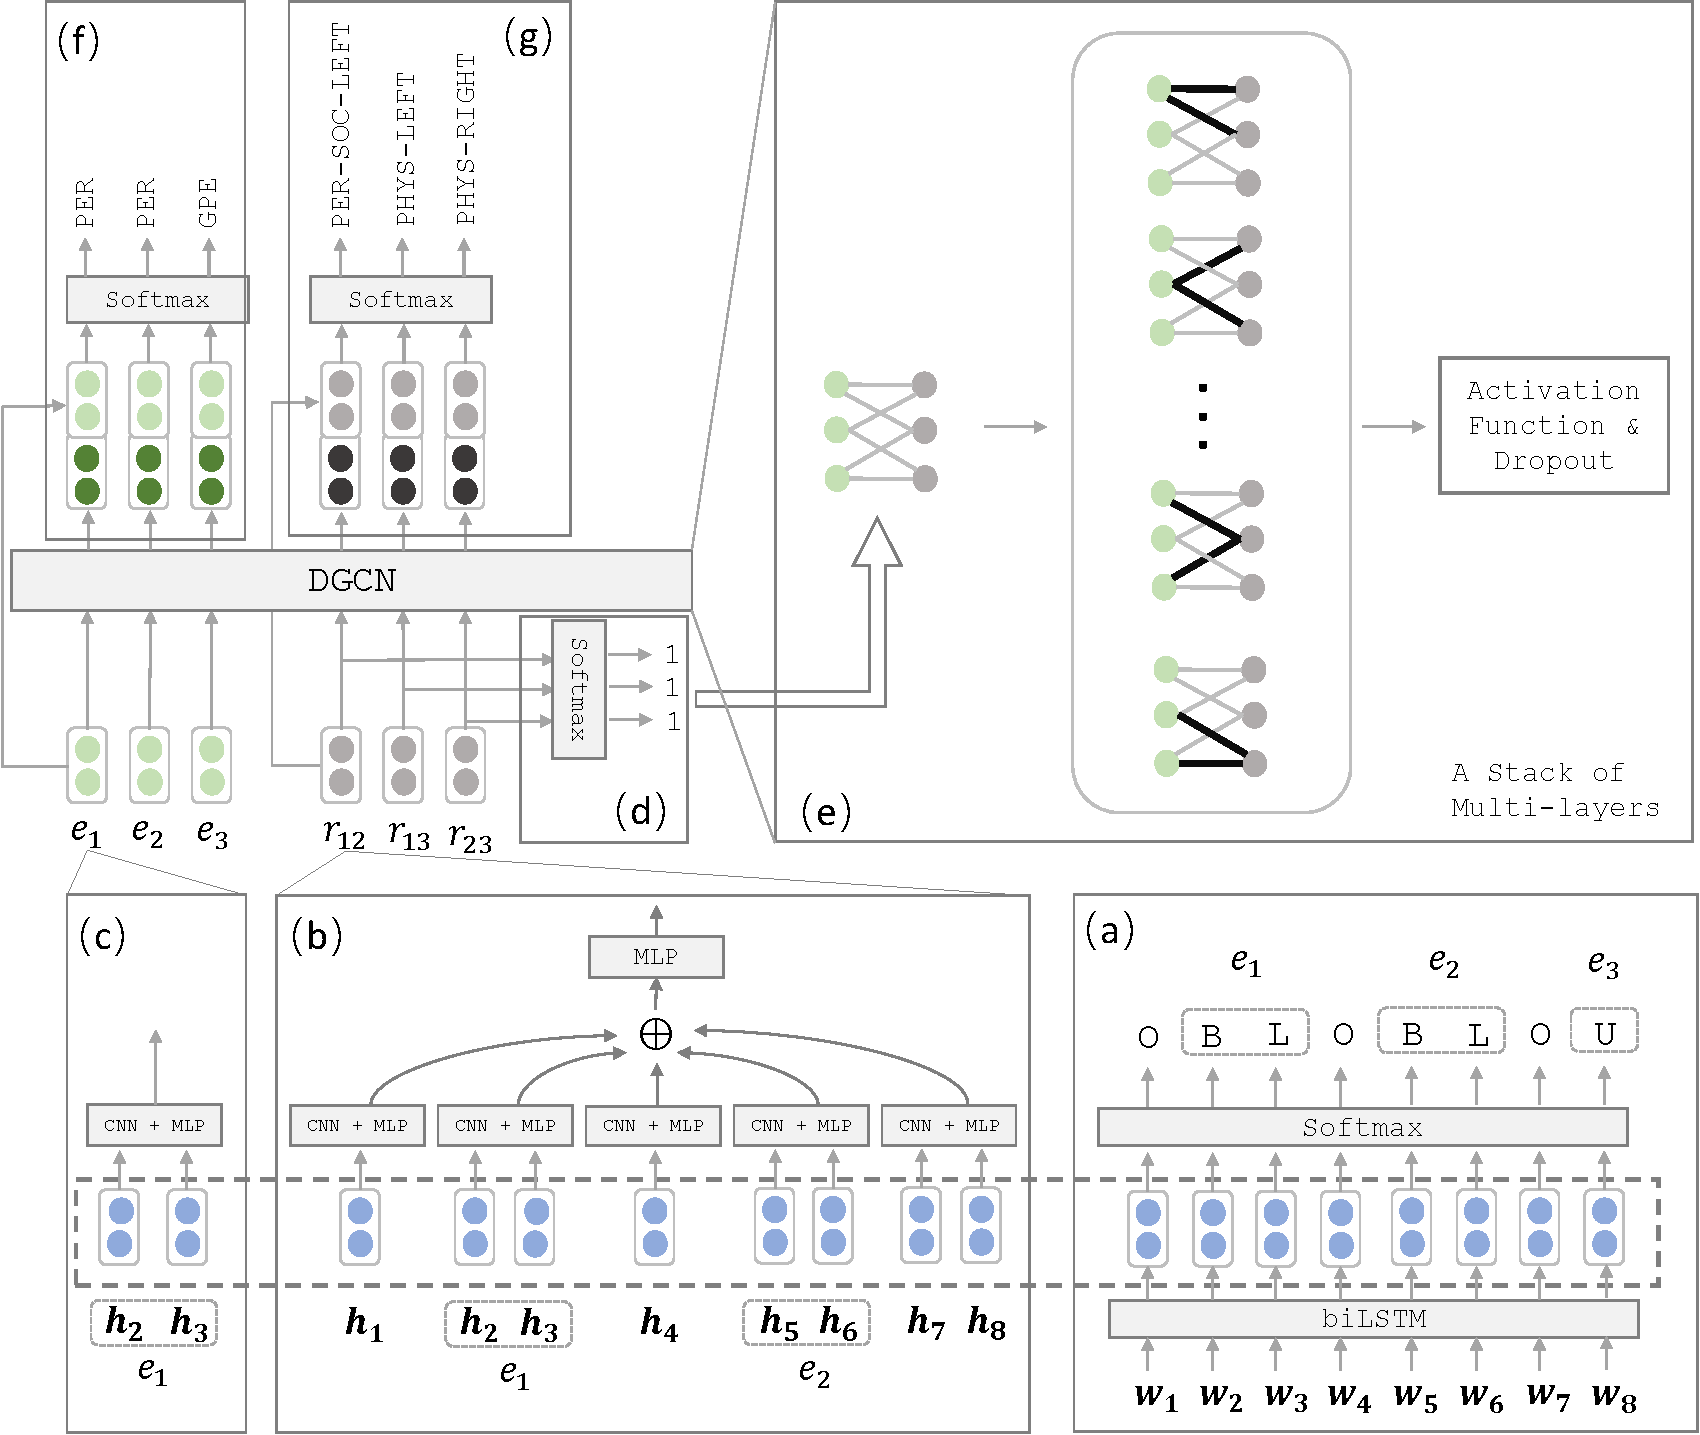
\includegraphics[width=5.0in]{../images/fig-model.pdf}
%    \end{center}
%    \caption{Our network structure for joint entity and relation extraction.}
%    \label{fig:net}
%\end{figure*}
\subsection{Entity Span Detection} \label{section:ent_span}
To extract entity spans from a sentence (Figure \ref{fig:ent-span}),
we adopt the \texttt{BILOU} sequence tagging scheme: 
\texttt{B}, \texttt{I}, \texttt{L} and \texttt{O} denote the begin,
inside, last and outside of a target span,
\texttt{U} denotes a single word span.
For example, for a person (\texttt{PER}) entity ``Patrick McDowell'', 
we assign \texttt{B} to ``Patrick'' and \texttt{L} to ``McDowell''.

Given an input sentence $s$,
we use a bidirectional long short term memory (biLSTM) network  \cite{DBLP:journals/neco/HochreiterS97} with parameter $\theta_\mathrm{seq}$
to incorporate information from both forward and backward directions of $s$.
\begin{IEEEeqnarray}{l}
    \mathbf{h}_i = \mathrm{biLSTM}(\mathbf{x}_i; \theta_\mathrm{seq}), \label{eq:bilstm}
\end{IEEEeqnarray}
where $\mathbf{h}_i$ is the concatenation of a forward and a backward LSTM's hidden states at position $i$,
and $\mathbf{x}_i$ is the word representation of $w_i$
which contains pre-trained embeddings and
character-based word representations
generated by running a CNN on the character sequences of $w_i$.
Then, we employ a softmax output layer to predict $w_i$'s tag $\hat{t}_i$,
\begin{IEEEeqnarray*}{c}
    \label{eq:ent_span_prob}
    P(\hat{t}_i|s)=\mathrm{Softmax}(\mathbf{W}_\mathrm{span}\mathbf{h}_i),
\end{IEEEeqnarray*}
where $\mathbf{W}_\mathrm{span}$ is the parameter. 
Given an input sentence $s$ and its gold tag sequence $\mathbf{t} = t_1, \dots, t_{|s|}$,
the training objective is to minimize
\footnote{We have also tried biLSTM-CRF \cite{DBLP:journals/corr/HuangXY15} 
as an advanced sequence labelling model, 
but performances are nearly the same in our experiments.
}
\begin{IEEEeqnarray}{c}
    \mathcal{L}_\mathrm{span} = 
    -\frac{1}{|s|} \sum_{i=1}^{|s|} \log P(\hat{t}_i = t_i|s).
    \label{eq:loss_seq}
\end{IEEEeqnarray}

\begin{figure} 
    \begin{center}
        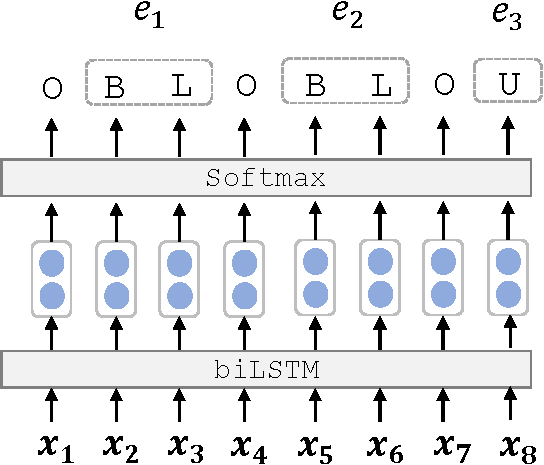
\includegraphics[width=2.5in]{../images/ent-span.pdf}
    \end{center}
    \caption{The biLSTM model for entity span detection.}
    \label{fig:ent-span}
\end{figure}

\subsection{Entity-Relation Bipartite Graph} \label{section:ent-rel-graph}

Given a set of detected entity spans $\hat{\mathcal{E}}$
(obtained from the entity span tag sequence $\hat{\mathbf{t}}$),
we consider all entity span pairs in $\hat{\mathcal{E}}$ as candidate relations
\footnote{The first entity span is always on the left side of the second entity span of each candidate relation, and we use in total $2\mathcal{T}_r+1$ relation types in order to consider both directions.
The additional type is the \texttt{None}  which means no relation between entity span pair.}.
Then we build a heterogeneous undirected bipartite graph $\mathcal{G}^s$ which contains entity nodes and relation nodes in a sentence $s$.
In the graph $\mathcal{G}^s$, interactions  on  multiple  entity types and relation types can be explicitly modeled. 
The number of nodes $n$ in the graph $\mathcal{G}^s$ is the number of entity spans
$|\hat{{\mathcal{E}}}|$ plus the number of all candidate relations $\frac{|\hat{{\mathcal{E}}}| (|\hat{{\mathcal{E}}}| - 1)}{2}$.
We have an initial input node embedding matrix $\mathbf{H}$.
For a relation $r_{12}$ and its two entities $e_1, e_2$,
we use $\mathbf{H}_{r_{12}}$ to denote relation embedding of $r_{12}$,
and use
$\mathbf{H}_{e_1}$,$\mathbf{H}_{e_2}$ to denote entity embedding of $e_1, e_2$ respectively.


\begin{figure*} 
    \begin{center}
        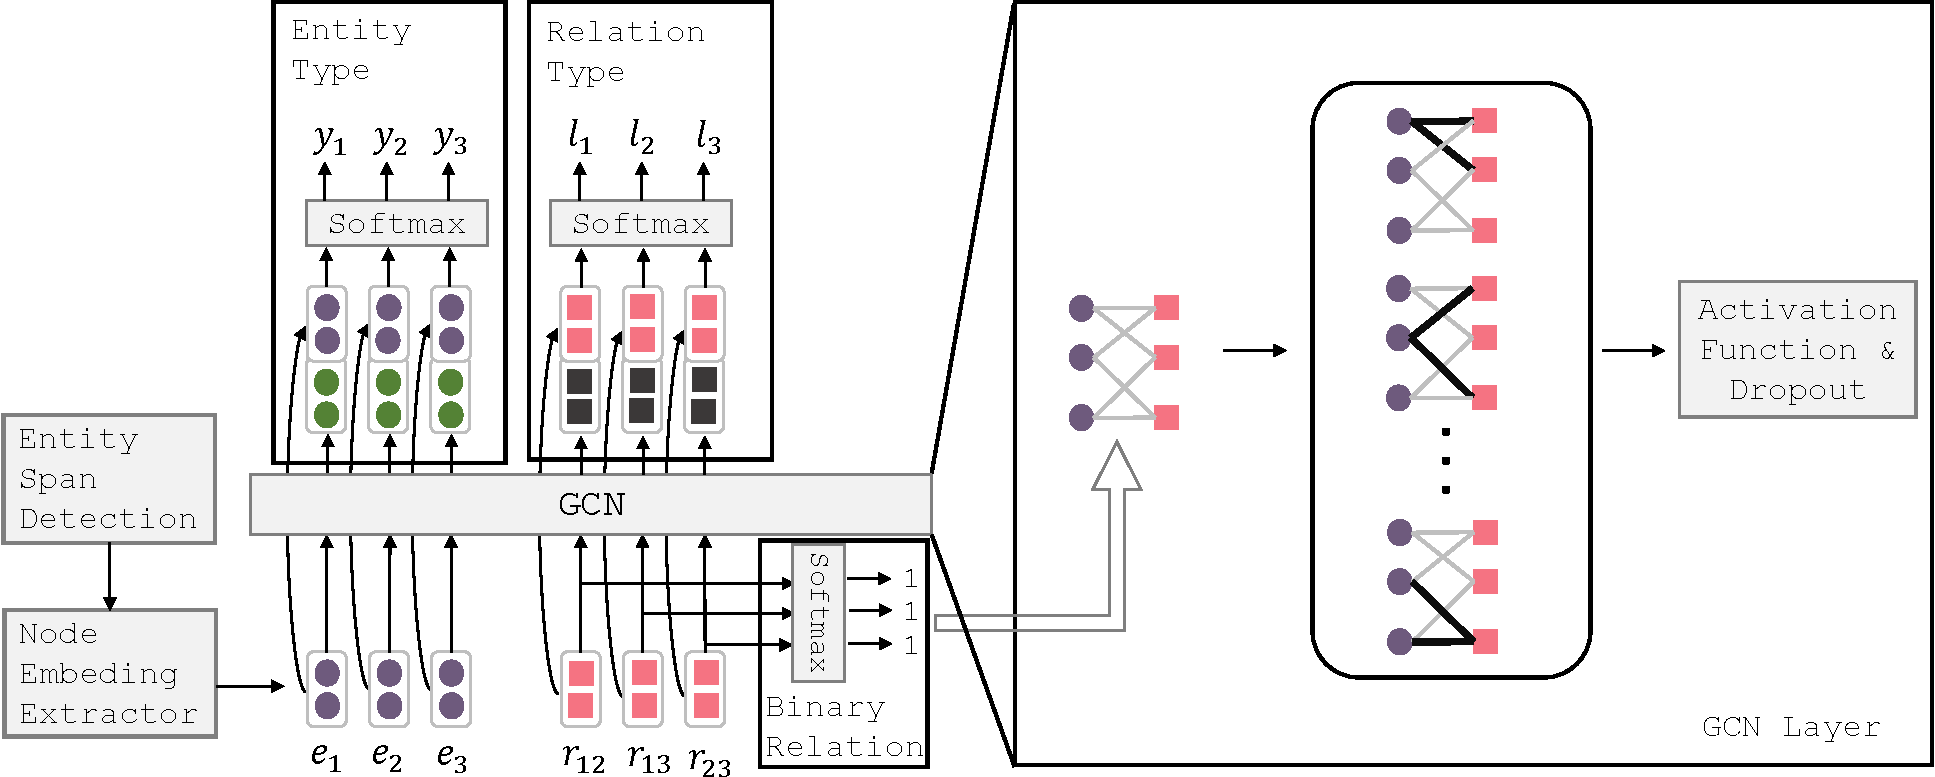
\includegraphics[width=6.0in]{../images/gcn.pdf}
    \end{center}
    \caption{Our network structure for the joint entity and relation extraction based on GCN. The node embedding extractor computes $\mathbf{H}_e$ and $\mathbf{H}_r$.}
    \label{fig:gcn}
\end{figure*}


Next, we build edges between entity nodes and relation nodes.
For graph edges,
we connect every relation node to its two entity nodes
instead of directly connecting any entity (relation) nodes.
Thus we focus on the bipartite graph.
The reasons are two folds. a) We do not think 
that all the remaining entities in the sentence are helpful.
Relation nodes are bridges between entity nodes and vice versa.
b) GCN is not suitable for fully-connected graphs  
because GCN reduce to rather trivial operations on fully-connected graphs.
It means that,
for an entity node $e$, the only way to observe other entities 
is through relations which $e$ takes part in.
For example, given a relation node $r_{12}$ and its two entity nodes $e_1, e_2$,
we add two edges. One is the edge between $e_1$ and $r_{12}$,
and another is the edge between $e_2$ and $r_{12}$.
We refer to it as \textbf{static} graph.

In order to further utilize the structure  of  the  graph (some kind of prior knowledge)
instead of using a static graph, 
we also investigate the \textbf{dynamic} graph for pruning redundant edges.
A key intuition is that if two entities hold a relation,
we could add two edges between the relation node and two entity nodes.
Conversely, if two entities have no relation,
we keep two entity nodes and the relation node separately.
To this end, we introduce the \textbf{binary relation classification} task.
It aims to predict whether a certain relation exists 
between an entity span pair (ignoring specific relation types).
We build a binary relation model which predicts a label in $\{0, 1\}$ 
to indicate the existence of a candidate relation 
based on relation node embedding.
Given a relation node $r_{ij}$ in a sentence $s$,
to get the posterior of the binary relation label $\hat{b}$,
we apply softmax layer on the relation node embedding $\mathbf{H}_{r_{ij}}$,
\begin{IEEEeqnarray*}{c}
    \label{eq:bin_rel_prob}
    P(\hat{b}| r_{ij}, s)=\mathrm{Softmax}(\mathbf{W}_\mathrm{bin}\mathbf{H}_{r_{ij}}),
\end{IEEEeqnarray*}
where $\mathbf{W}_\mathrm{bin}$ is the parameter.
The training objective is to minimize
\begin{IEEEeqnarray}{c}
    \mathcal{L}_{\mathrm{bin}} = - 
    \sum_{r_{ij}} 
    \frac{\log P(\hat{b} = b |r_{ij}, s)}
    {\mathrm{\#\ candidate\ relations}\ r_{ij}},
    \label{eq:loss_bin}
\end{IEEEeqnarray}
where true binary annotations $b$ are transformed from the original typed relation labels. Formally, the adjacency matrix $\mathbf{A}$  is defined as 
\begin{itemize}[leftmargin=*, itemindent=1pc]
    \item if $P(\hat{b} = 1 | r_{ij}, s) > 0.5$, we set the value of $\mathbf{A}$ between entity nodes $e_i, e_j$ and relation node $r_{ij}$ to 1.0,
    \item the diagonal elements of $\mathbf{A}$ are set to 1.0,
    \item while others are set to 0.0.
\end{itemize}

To compare with \textbf{hard} binary value $\mathbf{A}$,
we also try the \textbf{soft} value $\mathbf{A}$ in experiments.
It means that we set the value of $\mathbf{A}$ between entity nodes $e_i, e_j$ and relation node $r_{ij}$ 
to the probability $P(\hat{b} = 1 | r_{ij}, s)$ except for the diagonal elements (they are set to 1.0).

Here, we introduce how to compute two types of contextualized node embedding in the graph $\mathcal{G}^s$:
entity node embedding and relation node embedding.

\vspace{0.5em}
\noindent
\textbf{Entity Node Embedding}  
Given an entity span $e \in \hat{\mathcal{E}}$,
for each word $w_i \in e$,
we first collect $w_i$'s biLSTM hidden vector $\mathbf{h}_i$ from entity span model.
Then, we use a CNN (a single convolution layer with a max-pooling layer) with a multi-layer perceptron (MLP)
on vectors $\{\mathbf{h}_i | w_i \in e \}$
to obtain the resulting $d$-dimensional entity span node embedding $\mathbf{H}_{e}$ ($\mathbf{H}$ is a matrix mentioned before in Section \ref{section:gcn}),
as shown in the left part of Figure \ref{fig:node}.

\vspace{0.5em}
\noindent
\textbf{Relation Node Embedding}
Given a candidate relation $r_{12}$, 
we extract two types of features,
namely, features regarding words in $e_1, e_2$ 
and features regarding contexts of the entity span pair $(e_1, e_2)$.
For features on words in $e_1, e_2$,
we simply use entity node  embedding $\mathbf{H}_{e_1}$ and $\mathbf{H}_{e_2}$.
For context features of the entity span pair $(e_1, e_2)$,
we build three feature vectors by looking at words
between $e_1$ and $e_2$, words on the left of the
pair and words on the right of the pair.
Similarly, we build three features by running another CNN with an MLP.
Finally, the five feature vectors are concatenated to a single vector.
To get $d$-dimensional relation node embedding $\mathbf{H}_{r_{12}}$, 
we apply an MLP on the single vector,
as shown in the right part of Figure \ref{fig:node}.
\begin{figure} 
    \begin{center}
        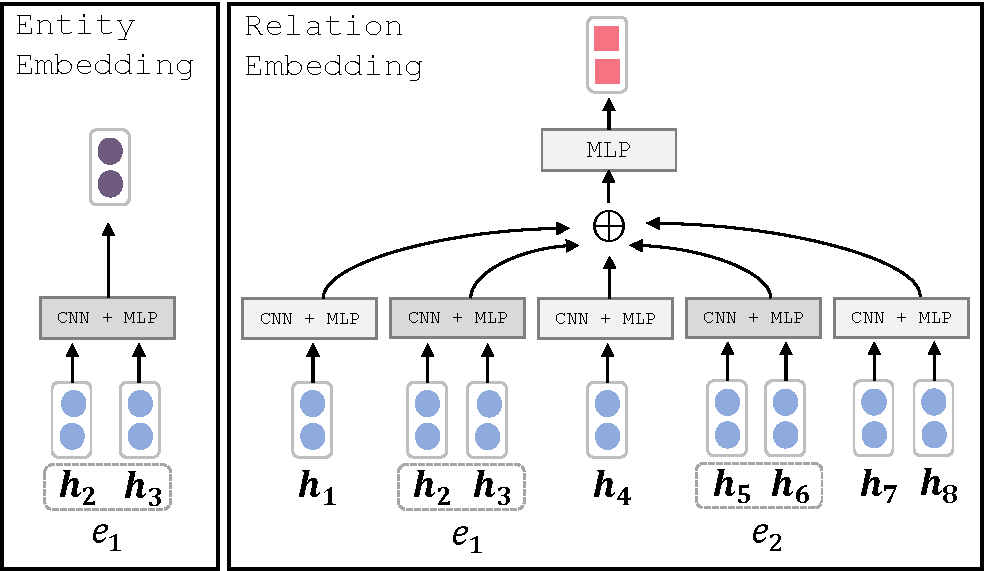
\includegraphics[width=3.0in]{../images/node-repr.pdf}
    \end{center}
    \caption{Our node embedding extractor.}
    \label{fig:node}
\end{figure}
\subsection{Joint Type Inference} \label{section:joint-type-inference}

After building the entity-relation bipartite graph,
we feed the graph into a multi-layer GCNs 
to obtain the node-level output $\mathbf{Z}$.
For each row in $\mathbf{Z}$ (entity or relation node representation), 
it can gather and summarize information from other
nodes in the graph $\mathcal{G}^s$ although
there is no direct entity-entity or relation-relation edges in the graph.
Then the final node representation $\mathbf{F}$ of graph $\mathcal{G}^s$ is concatenated by 
the input node embedding $\mathbf{H}$ and the node-level output $\mathbf{Z}$ ($\mathbf{H}, \mathbf{Z}$ and $\mathbf{F}$ are matrices).

Given an entity node $e_i$ and a relation node $r_{ij}$,
to predict the corresponding node types,
we pass the resulted node representation  into two fully connected layer 
with a softmax function, respectively,
\begin{IEEEeqnarray*}{c}
    \label{eq:ent_prob}
    P(\hat{y}| e_i, s)=\mathrm{Softmax}(\mathbf{W}_\mathrm{ent}\mathbf{F}_{e_i}),
\end{IEEEeqnarray*}
\begin{IEEEeqnarray*}{c}
    \label{eq:rel_prob}
    P(\hat{l}| r_{ij}, s)=\mathrm{Softmax}(\mathbf{W}_\mathrm{rel}\mathbf{F}_{r_{ij}}),
\end{IEEEeqnarray*}
where $\mathbf{W}_\mathrm{ent}$, $\mathbf{W}_\mathrm{rel}$ are parameters.
And the training objective is to minimize
\begin{IEEEeqnarray}{c}
    \mathcal{L}_{\mathrm{ent}} = - \frac{1}{|\hat{\mathcal{E}}|}
    \sum_{e_i \in \hat{\mathcal{E}}} 
    \log P(\hat{y} = y |e_i, s),
    \label{eq:loss_ent}
\end{IEEEeqnarray}

\begin{IEEEeqnarray}{c}
    \mathcal{L}_{\mathrm{rel}} = - 
    \sum_{r_{ij}} 
    \frac{\log P(\hat{l} = l |r_{ij}, s)}
    {\mathrm{\#\ candidate\ relations}\ r_{ij}},
    \label{eq:loss_rel}
\end{IEEEeqnarray}
where the true label $y, l$ can be read from annotations,
as shown in Figure \ref{fig:gcn}.

\subsection{Training}
To train the joint  model,
we optimize the combined objective function 
$\mathcal{L} = \mathcal{L}_\mathrm{span} + \mathcal{L}_\mathrm{bin} + \mathcal{L}_\mathrm{ent} +  \mathcal{L}_\mathrm{rel} $,
where the training is accomplished by the shared parameters.
We employ the scheduled sampling strategy
\cite{bengio2015scheduled}
in the entity model similar to
\cite{miwa-bansal:2016:P16-1}.
We optimize our model using Adadelta \cite{zeiler2012adadelta}
with gradient clipping.
The network is regularized with dropout.
Within a fixed number of epochs,
we select the model according to the best relation performance
on development sets\footnote{
Our word embeddings is initialized
with 100-dimensional glove \cite{pennington-socher-manning:2014:EMNLP2014} word embeddings.
The dimensionality of the hidden units and node embedding are set to 128.
For all CNN in our network, 
the kernel sizes are 2 and 3, 
and the output channels are 25.}.